\section{Methods}
\label{methods}
%From ILO:
%"Plan and carry out a small-scale investigation of an algorithmic research problem. This investigation could be theoretical, experimental, or both."
This section will cover which methods have been used throughout the project and why the methods have been chosen. Each method is motivated to support the problem definition and the analysis of the \qs{} implementation. The analysis consists of verifying the correctness of the stated results and applying the implementation with other data inputs to verify the relation between \qs{} and the baseline. Furthermore a number of practical tests are conducted to research possible performance gains.

\subsection{Experiment verification}

\subsubsection{Baseline comparison}
The paper compares the \qs{} performance with other compression algorithms, including (\pq{}) and a simple baseline algorithm, \gr{}. In order to verify their results, a version of Grid has been implemented as baseline to use for replication experiments. The basic concept is to make a range of buckets over each dimension for the point set. Each point will have its value for a dimension reduced to the value of the bucket in which the points value lies. By doing so, the value of the point can be stored with fewer bits and thus compress the data set.

\subsubsection{Other datasets}
To ensure proper verification of the results for the \qs{}, the implementation and baseline is tested on another dataset not included in the paper. If the results from another dataset somewhat match the results given in the paper \cite{wagner17}, it will strengthen the credibility of the practical efficiency of the \qs{} implementation.
\\
\\
The choice of other datasets could provide some additional insight into how the properties of some dataset might impact the optimality of the parameters given to the \qs{}. It might be interesting to feed datasets with different properties to the \qs{}, as results may change from very sparse / spread out datasets to very dense datasets.

\subsection{Experimenting with possible improvements}
A number of experiments will be conducted using different approaches to hopefully obtain improvements to the \qs{}. The approaches and experiments will be elaborated below.
%EMil vil gerne have "on" med

\subsubsection{Parameter heuristics}
In the current state the \qs{} has been run with a range of parameters and the results have been analyzed in order to obtain an understanding of which parameters gave the best results for the four presented datasets. To avoid conducting trial runs and result analysis to obtain the optimal parameters for some dataset, it would be desirable to have some heuristics approaching optimal or good parameters for the \qs{} given some dataset.

\subsubsection{Replacement bits}
In the pruning step bits are currently replaced with zero's. This effectively moves the pruned points in a certain direction and causes distortion. Instead of only introducing zero's into the bit string as replacement, inserting random bits might reduce the amount of distortion by pulling the point in different directions for each dimension rather than only distorting it in one direction. Another option could be to insert one's instead of zero's for certain datasets. 
%TODO: Figur der viser hvordan 0'er trækker points i en retning


\subsubsection{Synthetic dataset: \clust{}}
A synthetic dataset has been generated, with the goal to illustrate a scenario where \qsr{} in practice \textit{should} perform better than \qs{}. It is called \clust{}, as it contains four clusters of rather dense data points in Euclidean space. The clusters' centroids are programmed to be in each "corner" of the dataset(i.e. far apart). A simple illustration of this is presented in figure \ref{fig:clusters}, showing four clusters with each three points in 2D space.

\begin{figure}[h]
	\centering
	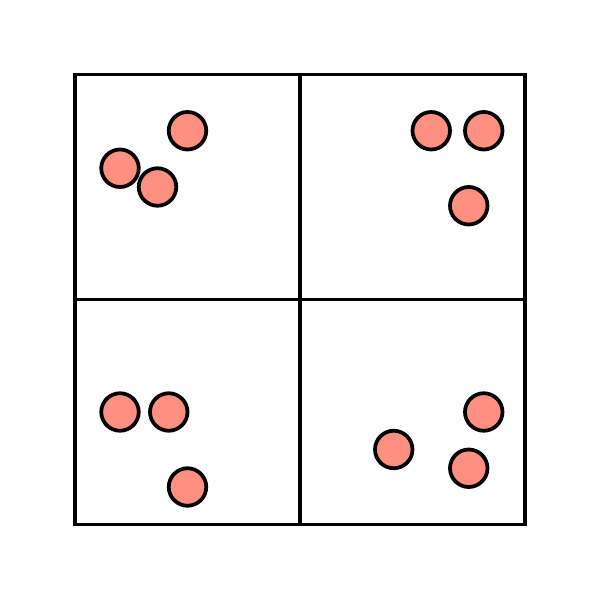
\includegraphics[scale=0.5]{figures/Clusters_example.png}
	\caption{Example of \clust{} in 2D space}
	\label{fig:clusters}
\end{figure}


\texttt{gen.cpp} is implemented to generate a dataset with such four clusters, taking as parameters the number of points, dimensions, and queries, as well as the minimum and maximum value in the dataset(which is the main factor for the resulting aspect ratio). The C++ library \texttt{normal\_distribution}\footnote{http://www.cplusplus.com/reference/random/normal\_distribution/} is used to randomly distribute the points in a cluster according to a \textit{normal distribution}, defined by a mean ($\mu$) with a specific standard deviation ($\sigma$). 

The generated set used for testing has 1,000,000 points, 128 dimensions and a resulting aspect ratio ($\Phi$) of 57.9, obtained from a minimum value of 100 and a maximum value of 600. 10,000 points (1\% of the dataset) are extracted to make up the query points. \clust{} are generated from two \texttt{normal\_distribution} generators fed with mean values of 162.5 and 537.5 respectively, and both with a standard deviation of 62.5.

\begin{table}[h]
\centering
\begin{tabular}{l l l l}
	\hline
	Dataset & Points & Dimensions & Aspect ratio ($\Phi$) \\
	\hline
	SIFT & 1,000,000 & 128 & $\geq$ 83.2 \\
	MNIST & 60,000 & 784 & $\geq$ 9.2 \\
	\clust{} & 1,000,000 & 128 & 57.9 \\
%	GIST & 1,000,000 & 960 & $\geq$ 580 \\
	\hline
\end{tabular}
\caption{Properties of the datasets}
\label{tab:datasets}
\end{table}

\clearpage